The cost function is a mathematical formula that measures the error between the network's predicted
output and the actual target values across a dataset. 
\begin{remark}
    Some sources consider loss and cost to be synonyms, while others consider cost to refer to the 
    entire dataset or a batch of data.
\end{remark}
\subsection{Gradient-Based Learning}
As with linear models, the gradient-based learning is a foundamental training paradigm where model parameters
are iteratively adjusted to minimize a cost function $J(\theta)$ using the \textbf{gradient descent algorithm}: 
\begin{equation}
    \theta \leftarrow \theta - \eta \nabla_{\theta} J
\end{equation}
\noindent where $\eta$ is the learning rate.
\newline
What changes in NN is the fact that the non-linearities make $\mathbf{J}$ \textbf{non-convex}, as shown in 
Fig \ref{fig:gradient_based}, so gradient descent may stop in a minimum that is not the best one, and 
where it stops depends on the starting $\theta$. In conclusion, the initial parameters $\theta$ must be 
\textit{small} in order to start in a non-saturated range, and \textbf{random} because otherwise every
hidden unit would compute the same thing and receive the same update (random values break this symmetry).
\begin{figure}[H]
    \centering
    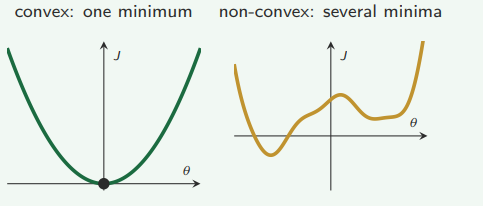
\includegraphics[width=0.7\linewidth]{immagini/gradient_based.png} 
    \caption{Difference between convex and non-convex}
    \label{fig:gradient_based}
\end{figure}
\noindent
One optimization of the gradient-descent algorithm is the 
\begin{definition}[Minibatch Stochastic Gradient Descent]
The algorithm is repeated until the validation error stops improving. At each step, the algorithm:
\begin{enumerate}
    \item Picks $m$ training examples at random to form a minibatch $\mathcal{B}$.
    \item Averages their gradients to compute $\hat{g} = \frac{1}{m} \sum_{i \in \mathcal{B}} 
    \nabla_{\theta} \ell(f(\mathbf{x}^{(i)}; \theta), y^{(i)})$, where individual gradients 
    are computed via back-propagation.
    \item Takes an optimization step: $\theta \leftarrow \theta - \eta \hat{g}$ using learning rate 
    $\eta$.
\end{enumerate}
\end{definition}
\noindent 
Here, $\hat{g}$ is a noisy but unbiased estimate of the true gradient $\nabla_{\theta} J$. 
A complete pass over all $n$ training examples is called an epoch. The noise of the estimate 
decreases as $1/\sqrt{m}$, with typical batch sizes ranging between $32$ and $512$ 
($32 \le m \le 512$).

\subsection{Maximum Likelihood}
The cost function comes from maximum likelihood, the network defines a 
\textbf{probability distribution} $p_{model}(y|\mathbf{x};\mathbf{\theta})$ over the possible targets. 
An advantage of this approach is that is not necessary to design cost functions for each model.
\begin{definition}[Maximum Likelihood]  
    choose $\theta$ so that the correct answers get high probability. In other words, minimize the average
    negative log-probability:
    \begin{equation}
        J(\theta) = -\frac{1}{n} \sum_{i=1}^{n} \log p_{\text{model}}(y^{(i)} \mid \mathbf{x}^{(i)}; \theta)
    \end{equation}
\end{definition}
An other form of this function is
\begin{equation}
    $$\begin{equation} J(\boldsymbol{\theta}) = -\mathbb{E}_{\mathbf{x},\mathbf{y}\sim\hat{p}_{\text{data}}} \log p_{\text{model}}(\boldsymbol{y} \mid \boldsymbol{x}). \end{equation}$$
\end{equation}
where $\hat{p}_{\text{data}}$ gives probability 1/n to each training pair. This is also called \textbf{Cross-Entropy}.
The negativity helps to avoid the problem of the saturation of the units of the NN.

\subsubsection{Derivation: A Gaussian Output Gives the Squared Error}
A practical application of this principle is choosing a Gaussian output distribution for the network, 
assuming the target is the network output plus Gaussian noise with variance $s^2$:
\begin{equation}
    p_{\text{model}}(y \mid \mathbf{x}) = \mathcal{N}(y; f(\mathbf{x}; \boldsymbol{\theta}), s^2) = \frac{1}{\sqrt{2\pi s^2}} \exp\left(-\frac{(y - f(\mathbf{x}; \boldsymbol{\theta}))^2}{2s^2}\right)
\end{equation}
Taking the negative log-probability yields:
\begin{equation}
    -\log p_{\text{model}}(y \mid \mathbf{x}) = \frac{1}{2s^2} (y - f(\mathbf{x}; \boldsymbol{\theta}))^2 + \frac{1}{2}\log(2\pi s^2)
\end{equation}
Since the last term does not depend on $\boldsymbol{\theta}$, minimizing the average negative 
log-likelihood over the dataset leads directly to the Mean Squared Error cost function:
\begin{equation}
    J(\boldsymbol{\theta}) = \frac{1}{2s^2} \cdot \frac{1}{n} \sum_{i} \left(y^{(i)} - f(\mathbf{x}^{(i)}; \boldsymbol{\theta})\right)^2 + \text{const}
\end{equation}
Thus, under a Gaussian assumption, maximum likelihood is equivalent to minimizing the squared error.
\newline
\textbf{Mean absolute or squared error} often lead to poor results when used with gradient-based 
optimization due to saturation.